\documentclass[12pt,titlepage]{article}
\usepackage[utf8]{inputenc}
\usepackage[a4paper, total={16cm, 22cm}]{geometry}
\usepackage[
	backend=biber,
	bibstyle=authoryear,
	citestyle=authoryear-comp,
	sorting=nyt,
	uniquename=false,
	maxbibnames=99
]{biblatex}
\usepackage{
	fancyhdr,
	amsmath,
	amssymb,
	graphicx,
	siunitx,
}


% \addbibresource{references.bib}

\setlength{\parskip}{1em}
\pagestyle{fancy}
\fancyhf{}
\rhead{Thomas Schanzer}
\lhead{}
\lfoot{\leftmark}
\rfoot{Page \thepage}
\setlength{\headheight}{15pt}
\renewcommand{\headrulewidth}{2pt}
\renewcommand{\footrulewidth}{1pt}
\fancypagestyle{first}{
	\fancyhead{}
	\fancyfoot{}
	\renewcommand{\headrulewidth}{0pt}
	\renewcommand{\footrulewidth}{0pt}
}

\begin{document}

% \includepdf[pages=-]{coversheet.pdf}

\begin{titlepage}
    \begin{center}
        
        \vspace{1cm} 
        \Huge
        \textbf{Title}
        
        \Large
        \textbf{Subtitle}
            
        \vspace{0.75cm}
            
        \textbf{Thomas D. Schanzer}
            
        \vspace{1.5cm}
            
        
\includegraphics[width=0.4\textwidth]{figures/unsw}

        \vspace{1cm}

        \large    
        Taste of Research 2021

        \vspace{1cm}
            
        \large
        School of Physics\\
        Faculty of Science\\
        University of New South Wales\\
        Sydney, Australia\\
        \vspace{0.5cm}
        Term 3 2021
        \vfil
            
    \end{center}
\end{titlepage}

\begin{center}
	\large
	\textbf{Abstract}
\end{center}

Abstract

\begin{center}
	\large
	\textbf{Acknowledgements}
\end{center}

Acknowledgements

\tableofcontents

\clearpage
\section{Introduction and theory}

\section{Literature review}

\section{Methods}

\section{Results}
\subsection{Entrainment reduces downdraft strength}

\begin{figure}[ht]
	\centering
	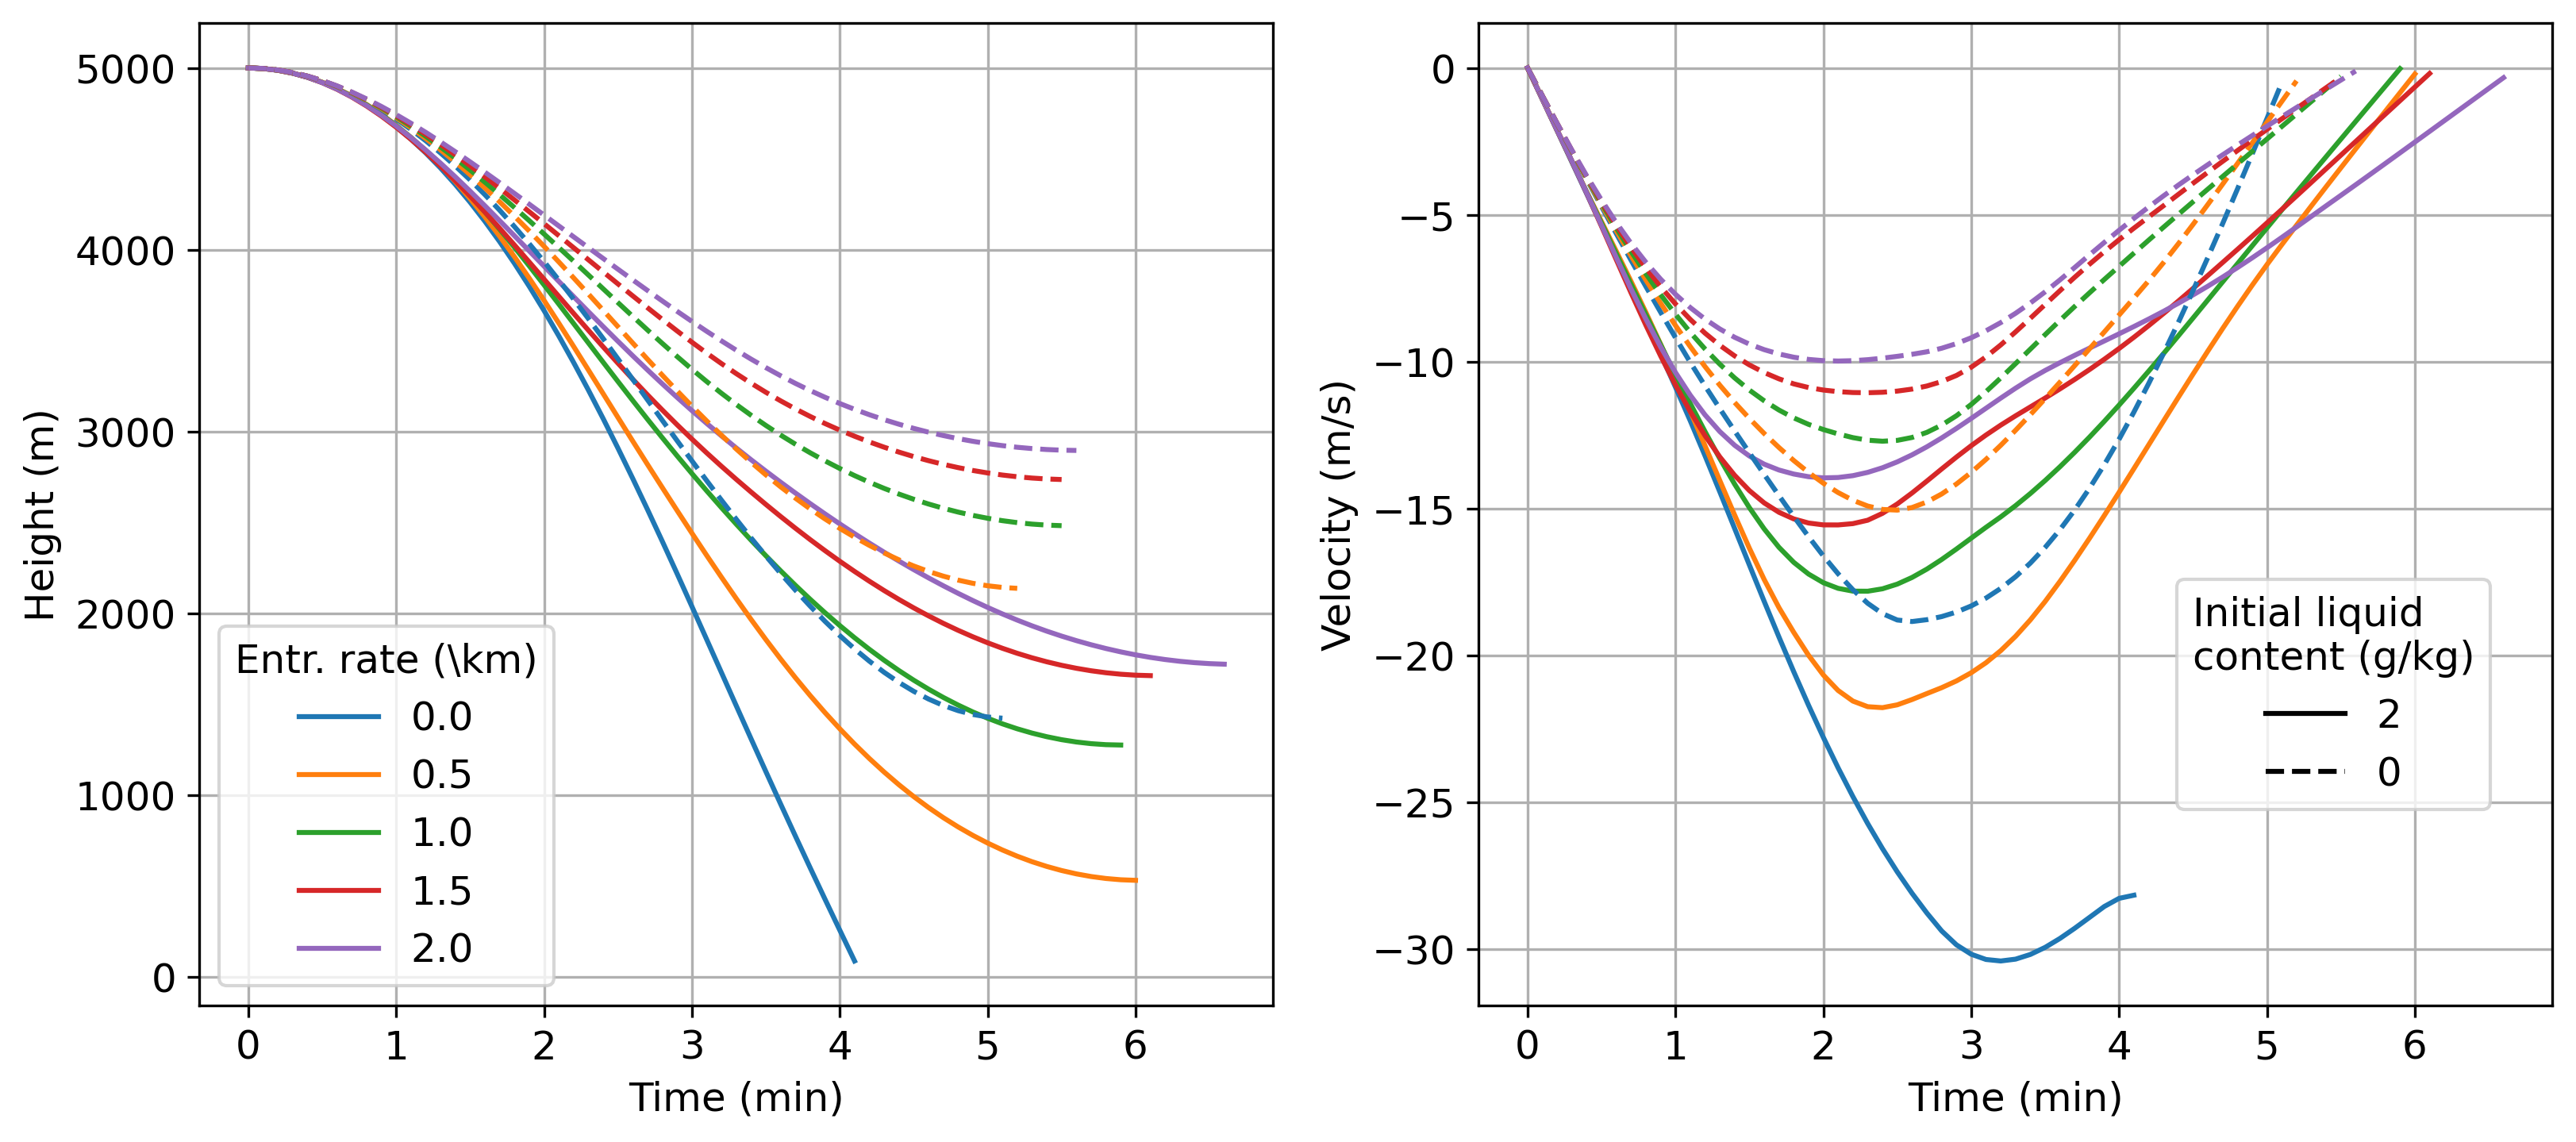
\includegraphics[width=0.8\linewidth]
		{figures/20211026_experiments_sydney/entrainment_rate_vs_motion}
	\caption{
		Height and velocity over time of a parcels, initial height
		$\SI{5}{\kilo\meter}$, that are initially cooled by evaporation to
		the point of saturation. We use sounding data from Sydney
		for the environmental temperature and dew point profiles.}
	\label{sydney_entrainment_rate_vs_motion}
\end{figure}

\begin{figure}[ht]
	\centering
	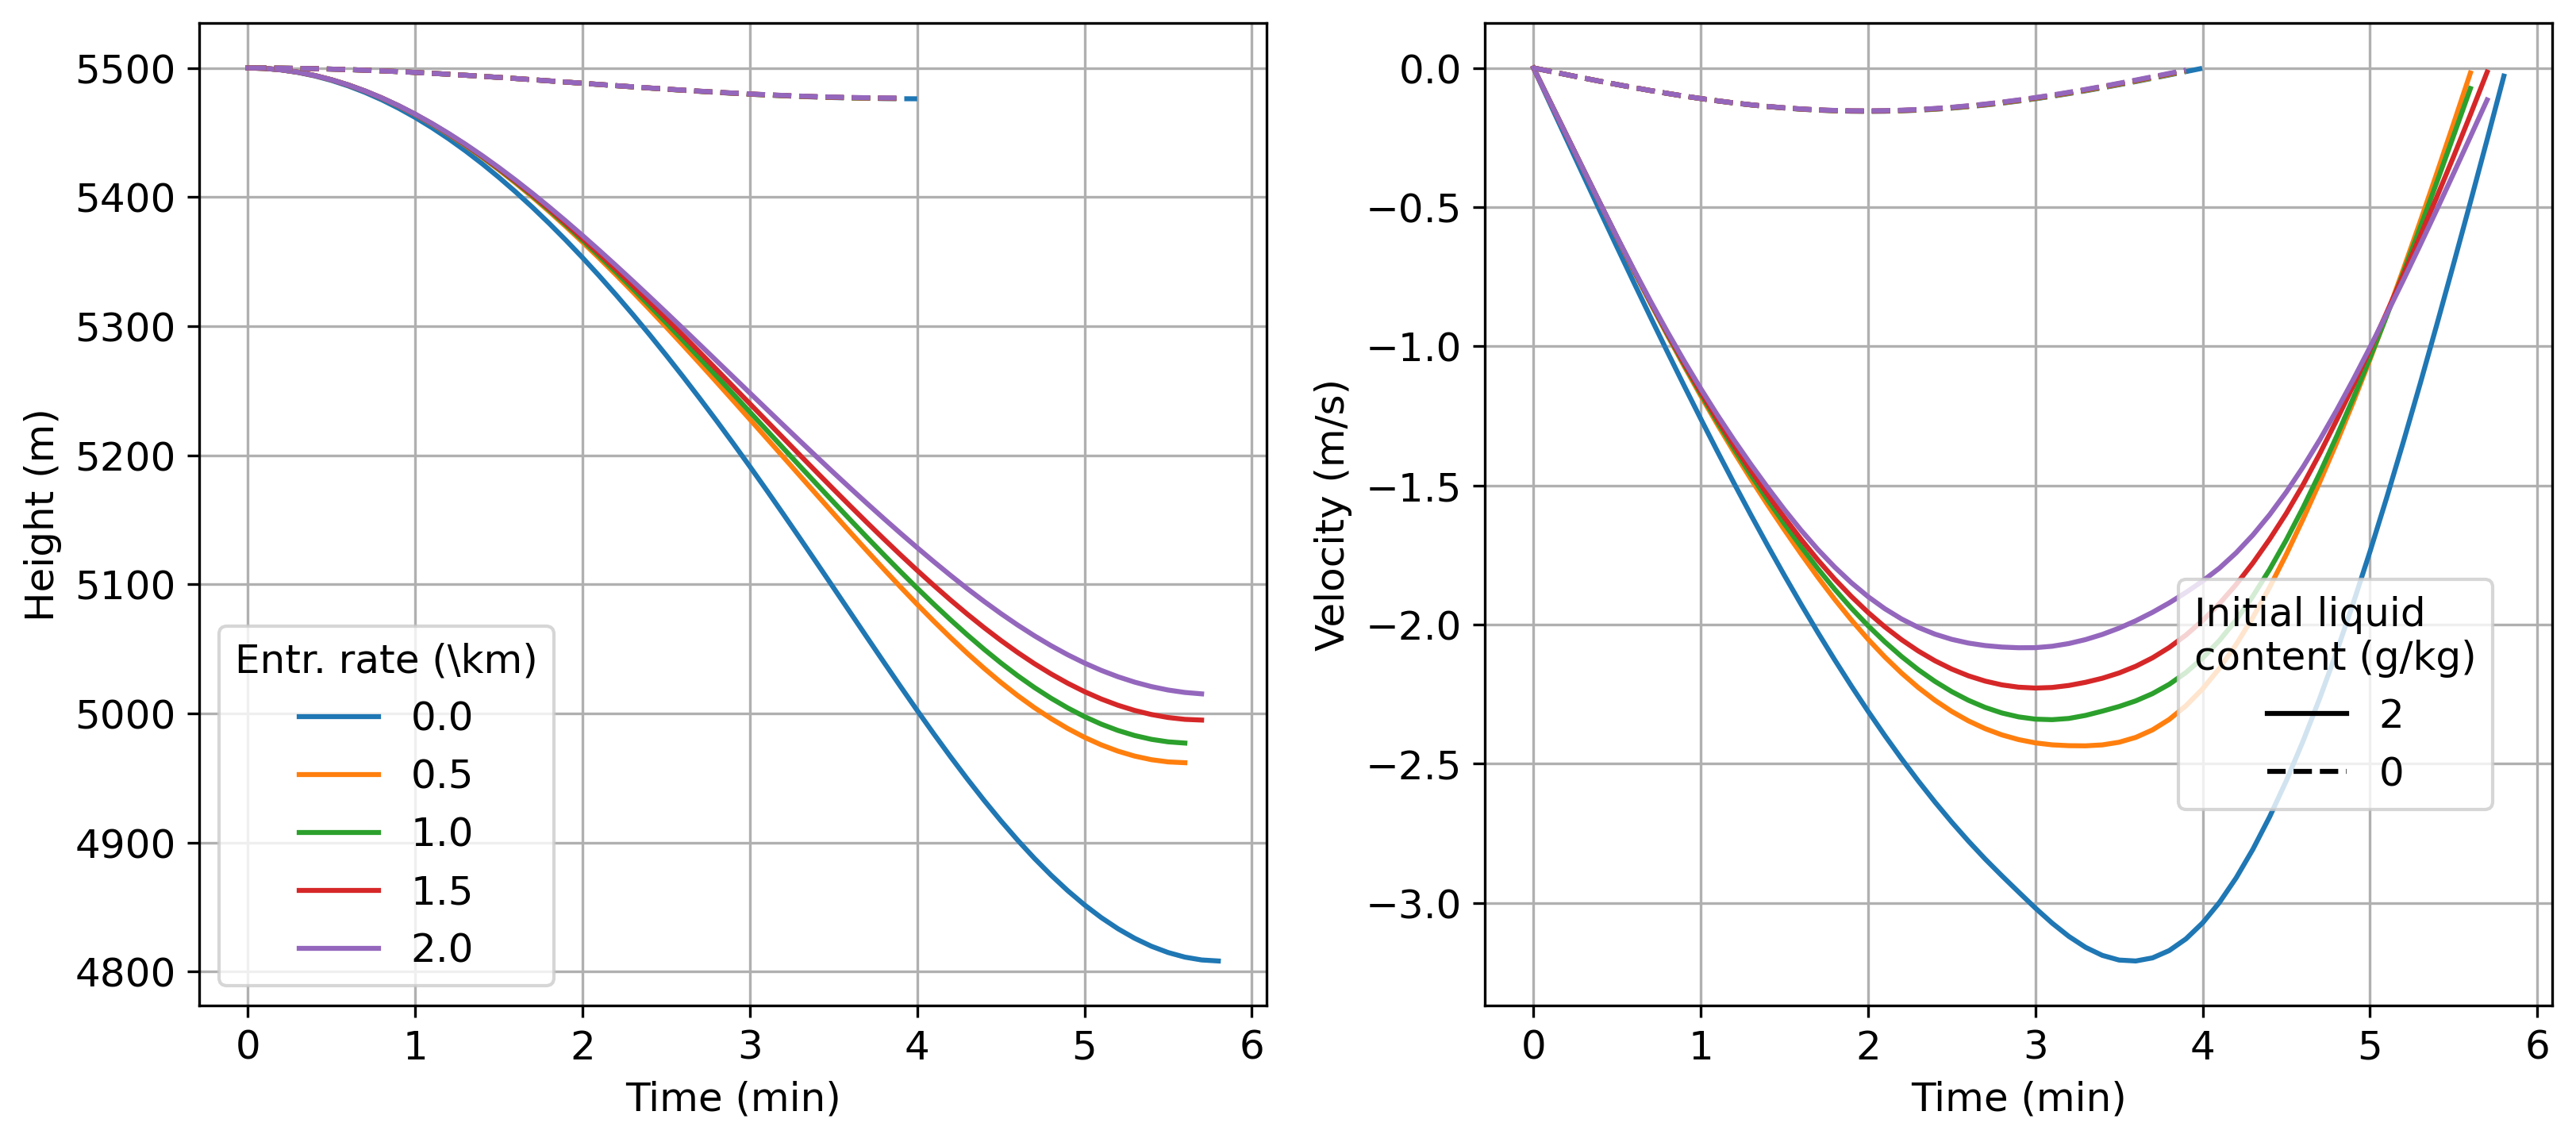
\includegraphics[width=0.8\linewidth]
		{figures/20211027_experiments_singapore/entrainment_rate_vs_motion}
	\caption{
		The results of the same calculation used for Figure
		\ref{sydney_entrainment_rate_vs_motion}, but using sounding data
		from Singapore for the environmental temperature and dew point
		profiles.}
	\label{singapore_entrainment_rate_vs_motion}
\end{figure}

\begin{figure}[ht]
	\centering
	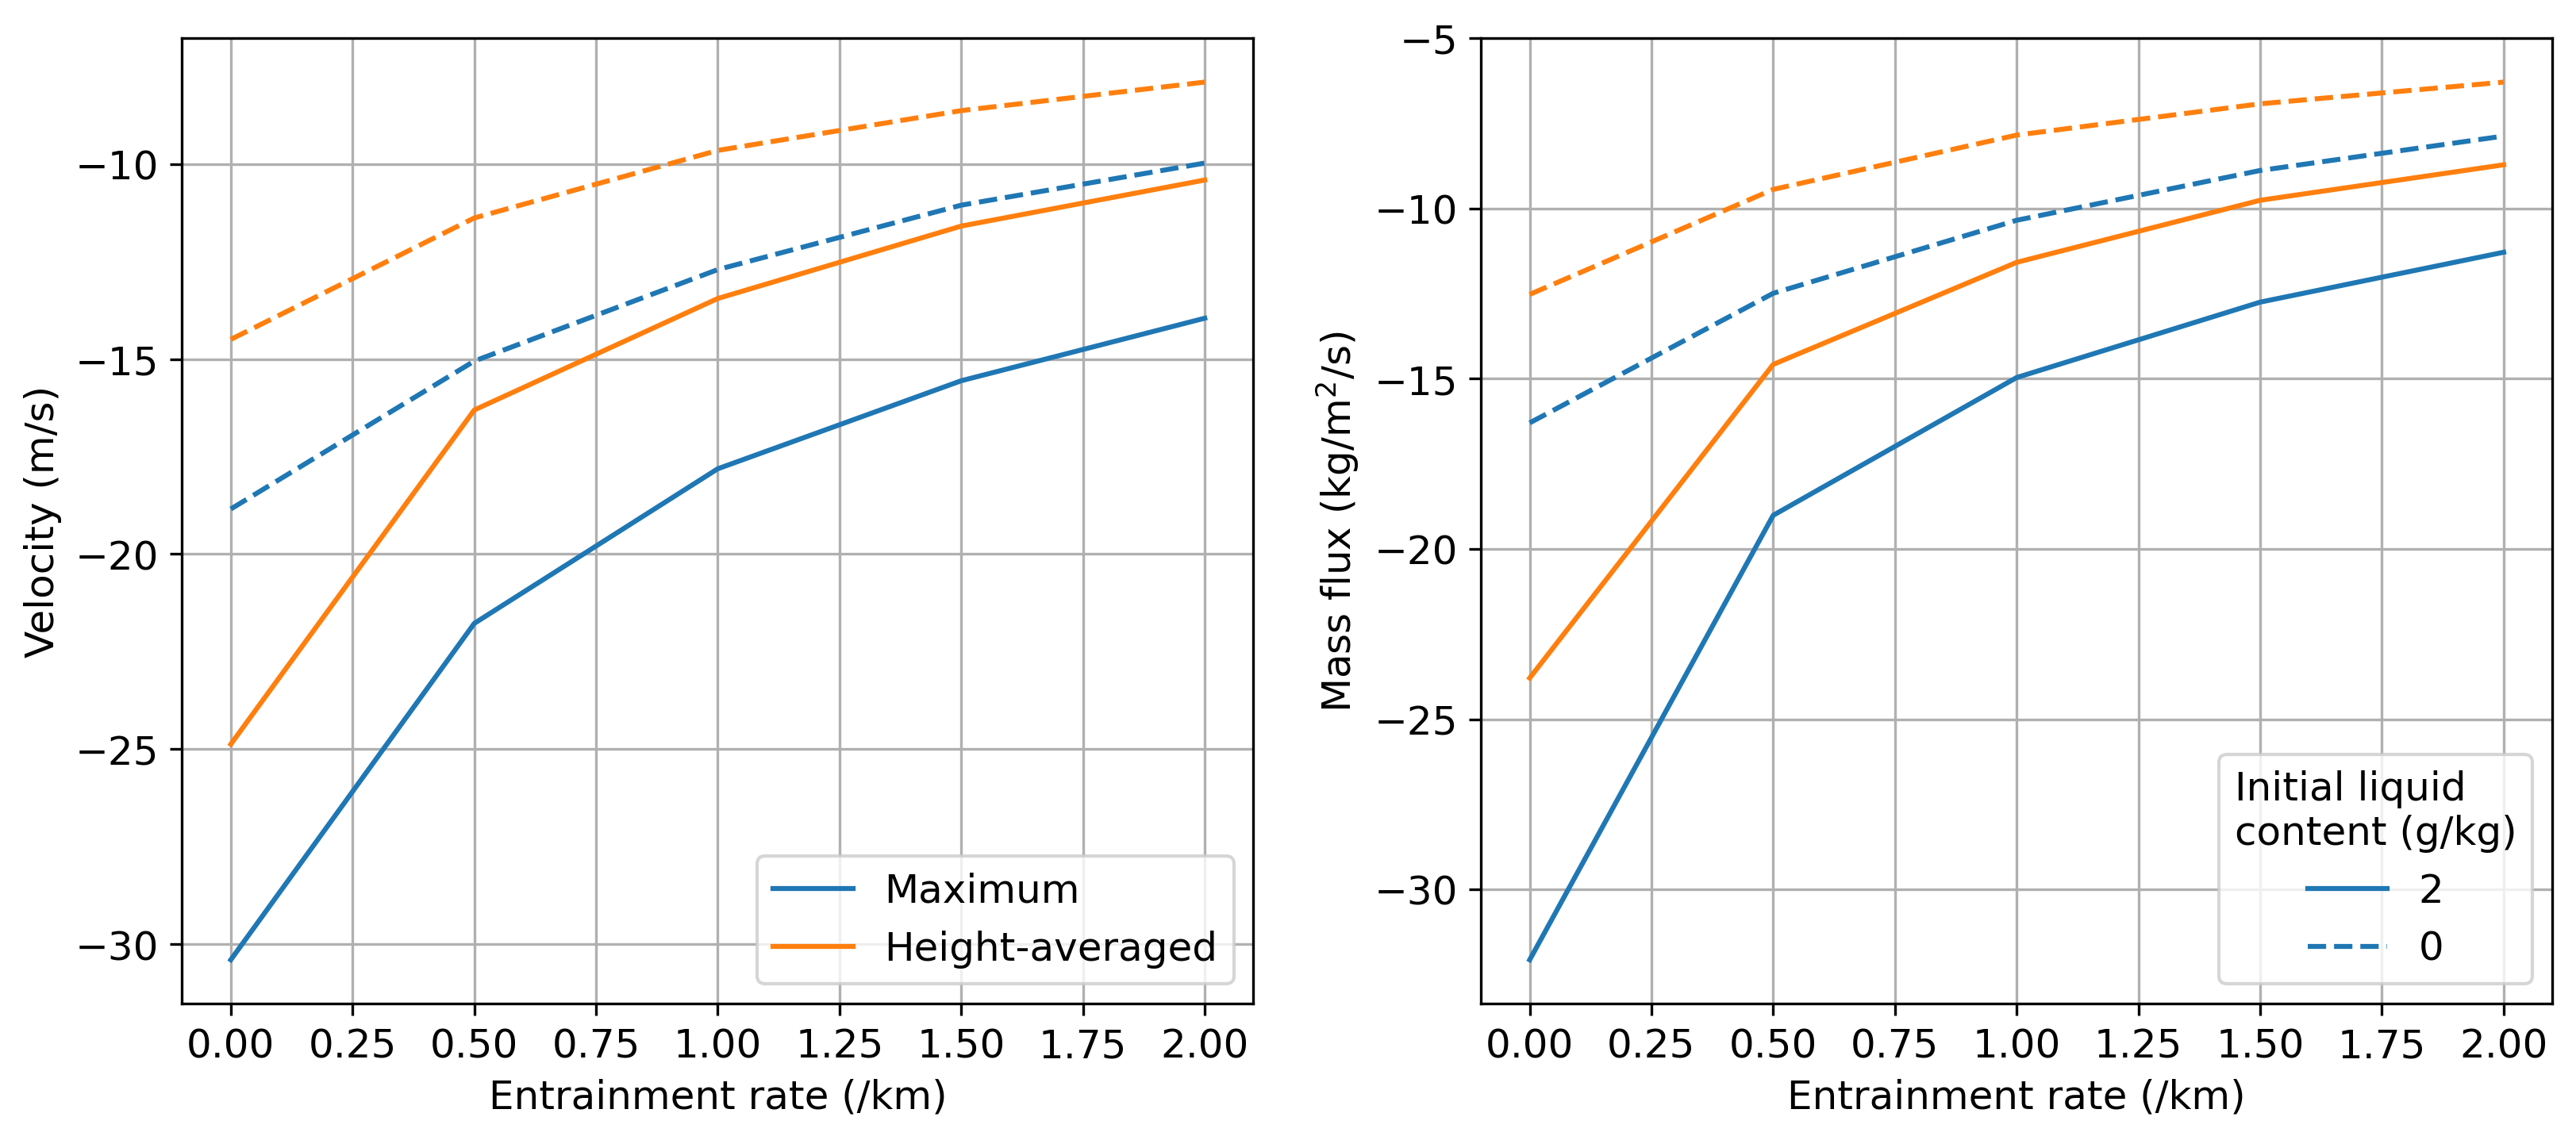
\includegraphics[width=0.8\linewidth]
		{figures/20211026_experiments_sydney/entrainment_rate_vs_velocity}
	\caption{
		Maximum and height-averaged downdraft velocities from Figure
		\ref{sydney_entrainment_rate_vs_motion}, (using Sydney sounding
		data).}
	\label{sydney_entrainment_rate_vs_velocity}
\end{figure}

\begin{figure}[ht]
	\centering
	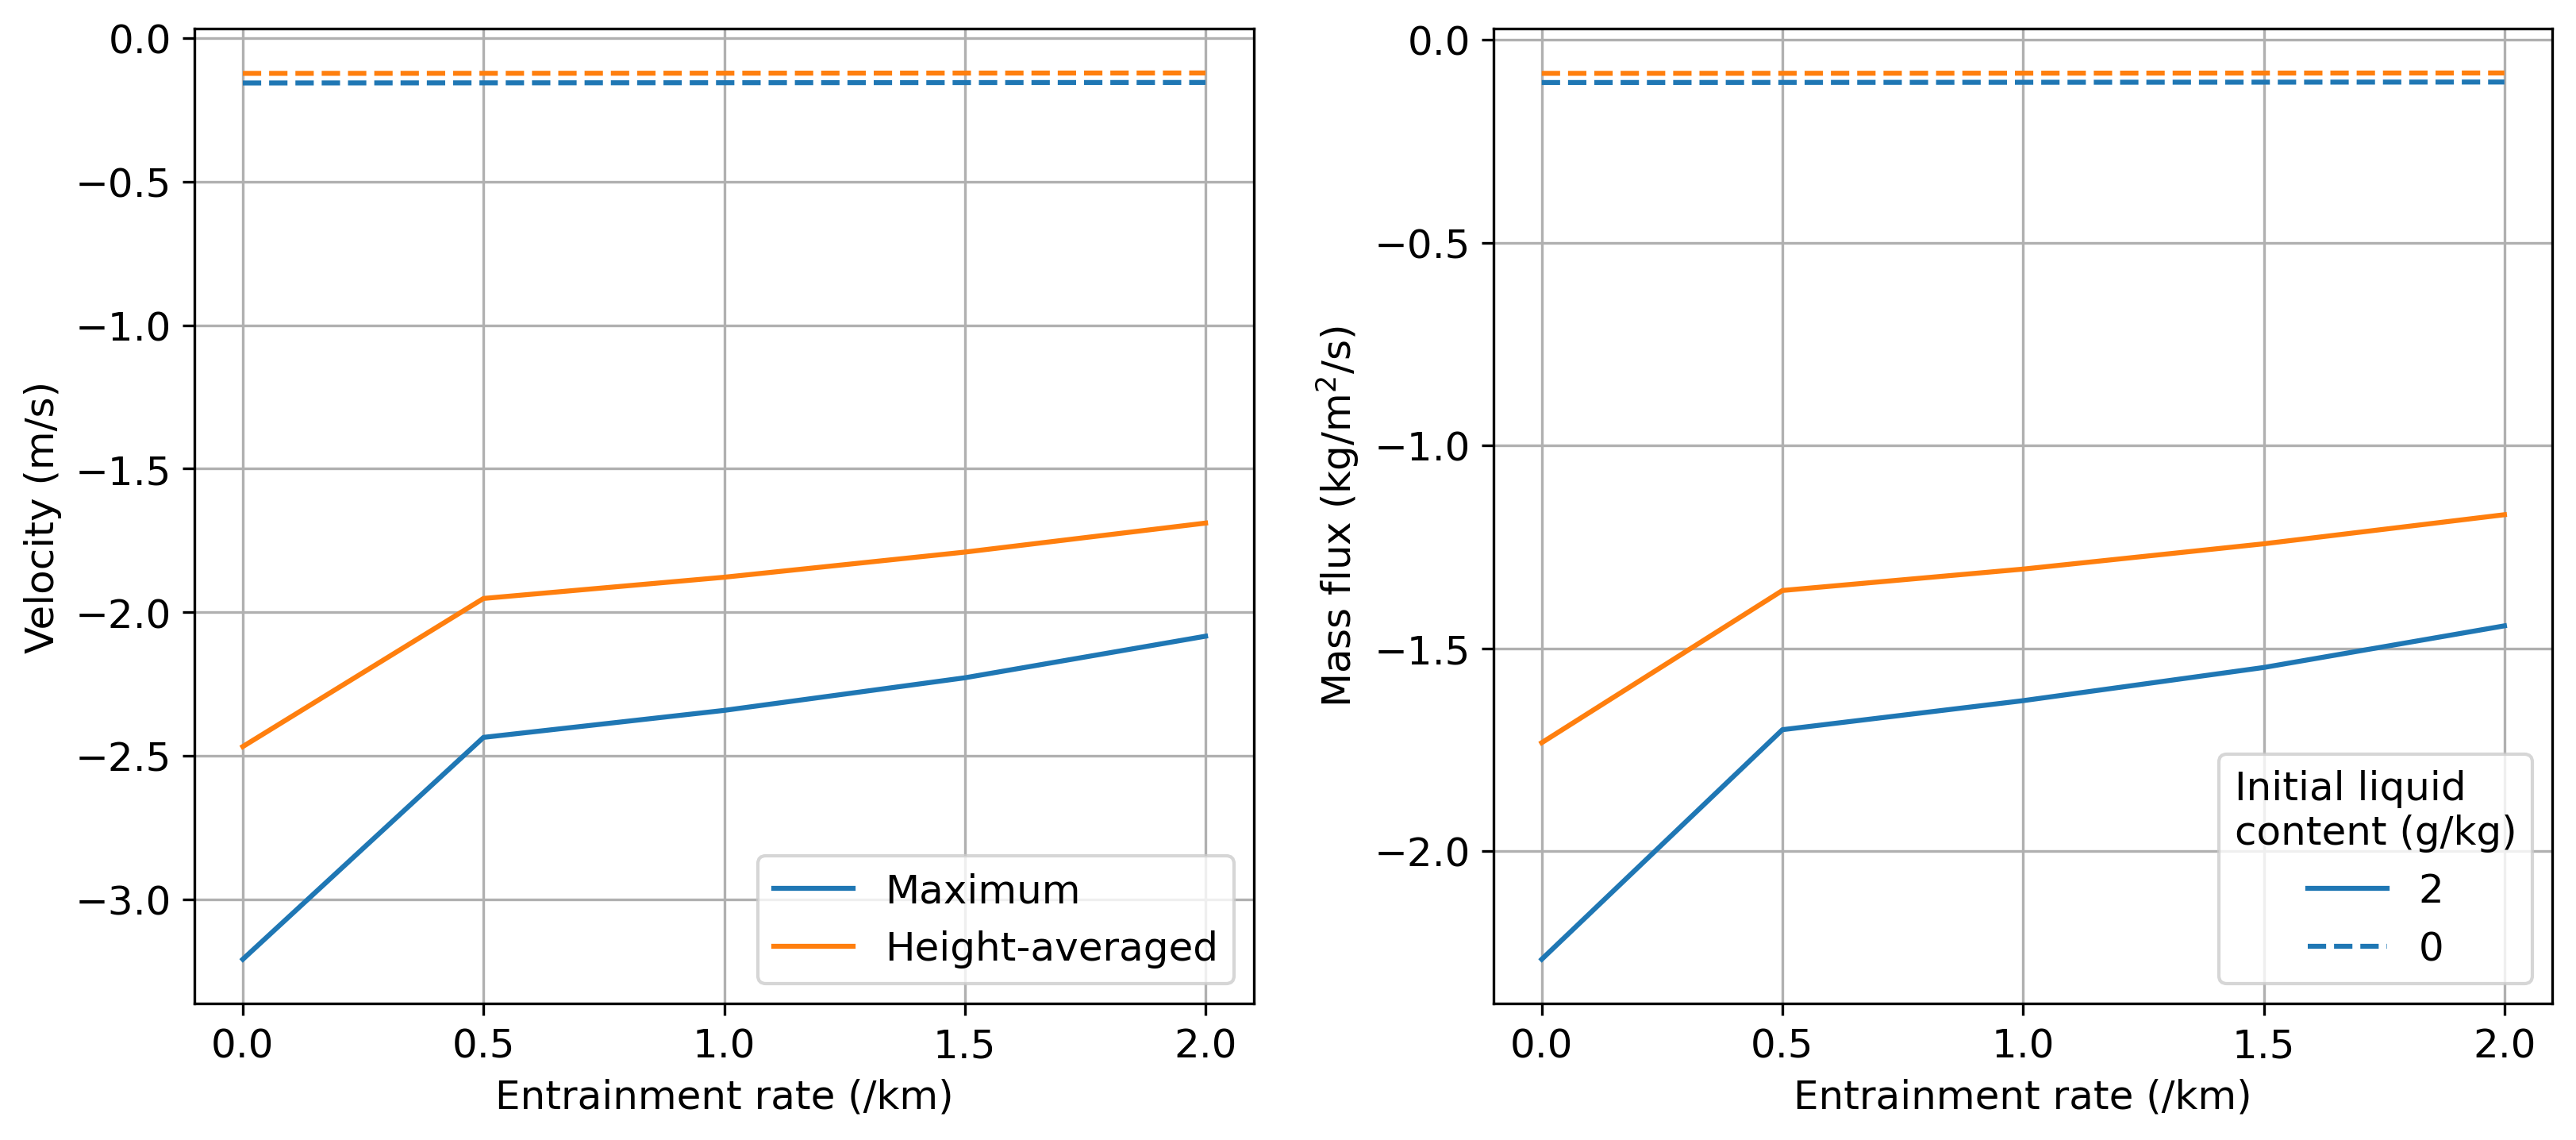
\includegraphics[width=0.8\linewidth]
		{figures/20211027_experiments_singapore/entrainment_rate_vs_velocity}
	\caption{
		Maximum and height-averaged downdraft velocities from Figure
		\ref{singapore_entrainment_rate_vs_motion}, (using Singapore sounding
		data).}
	\label{singapore_entrainment_rate_vs_velocity}
\end{figure}


\clearpage
\subsection{Initial addition of water increases downdraft strength}

\begin{figure}[ht]
	\centering
	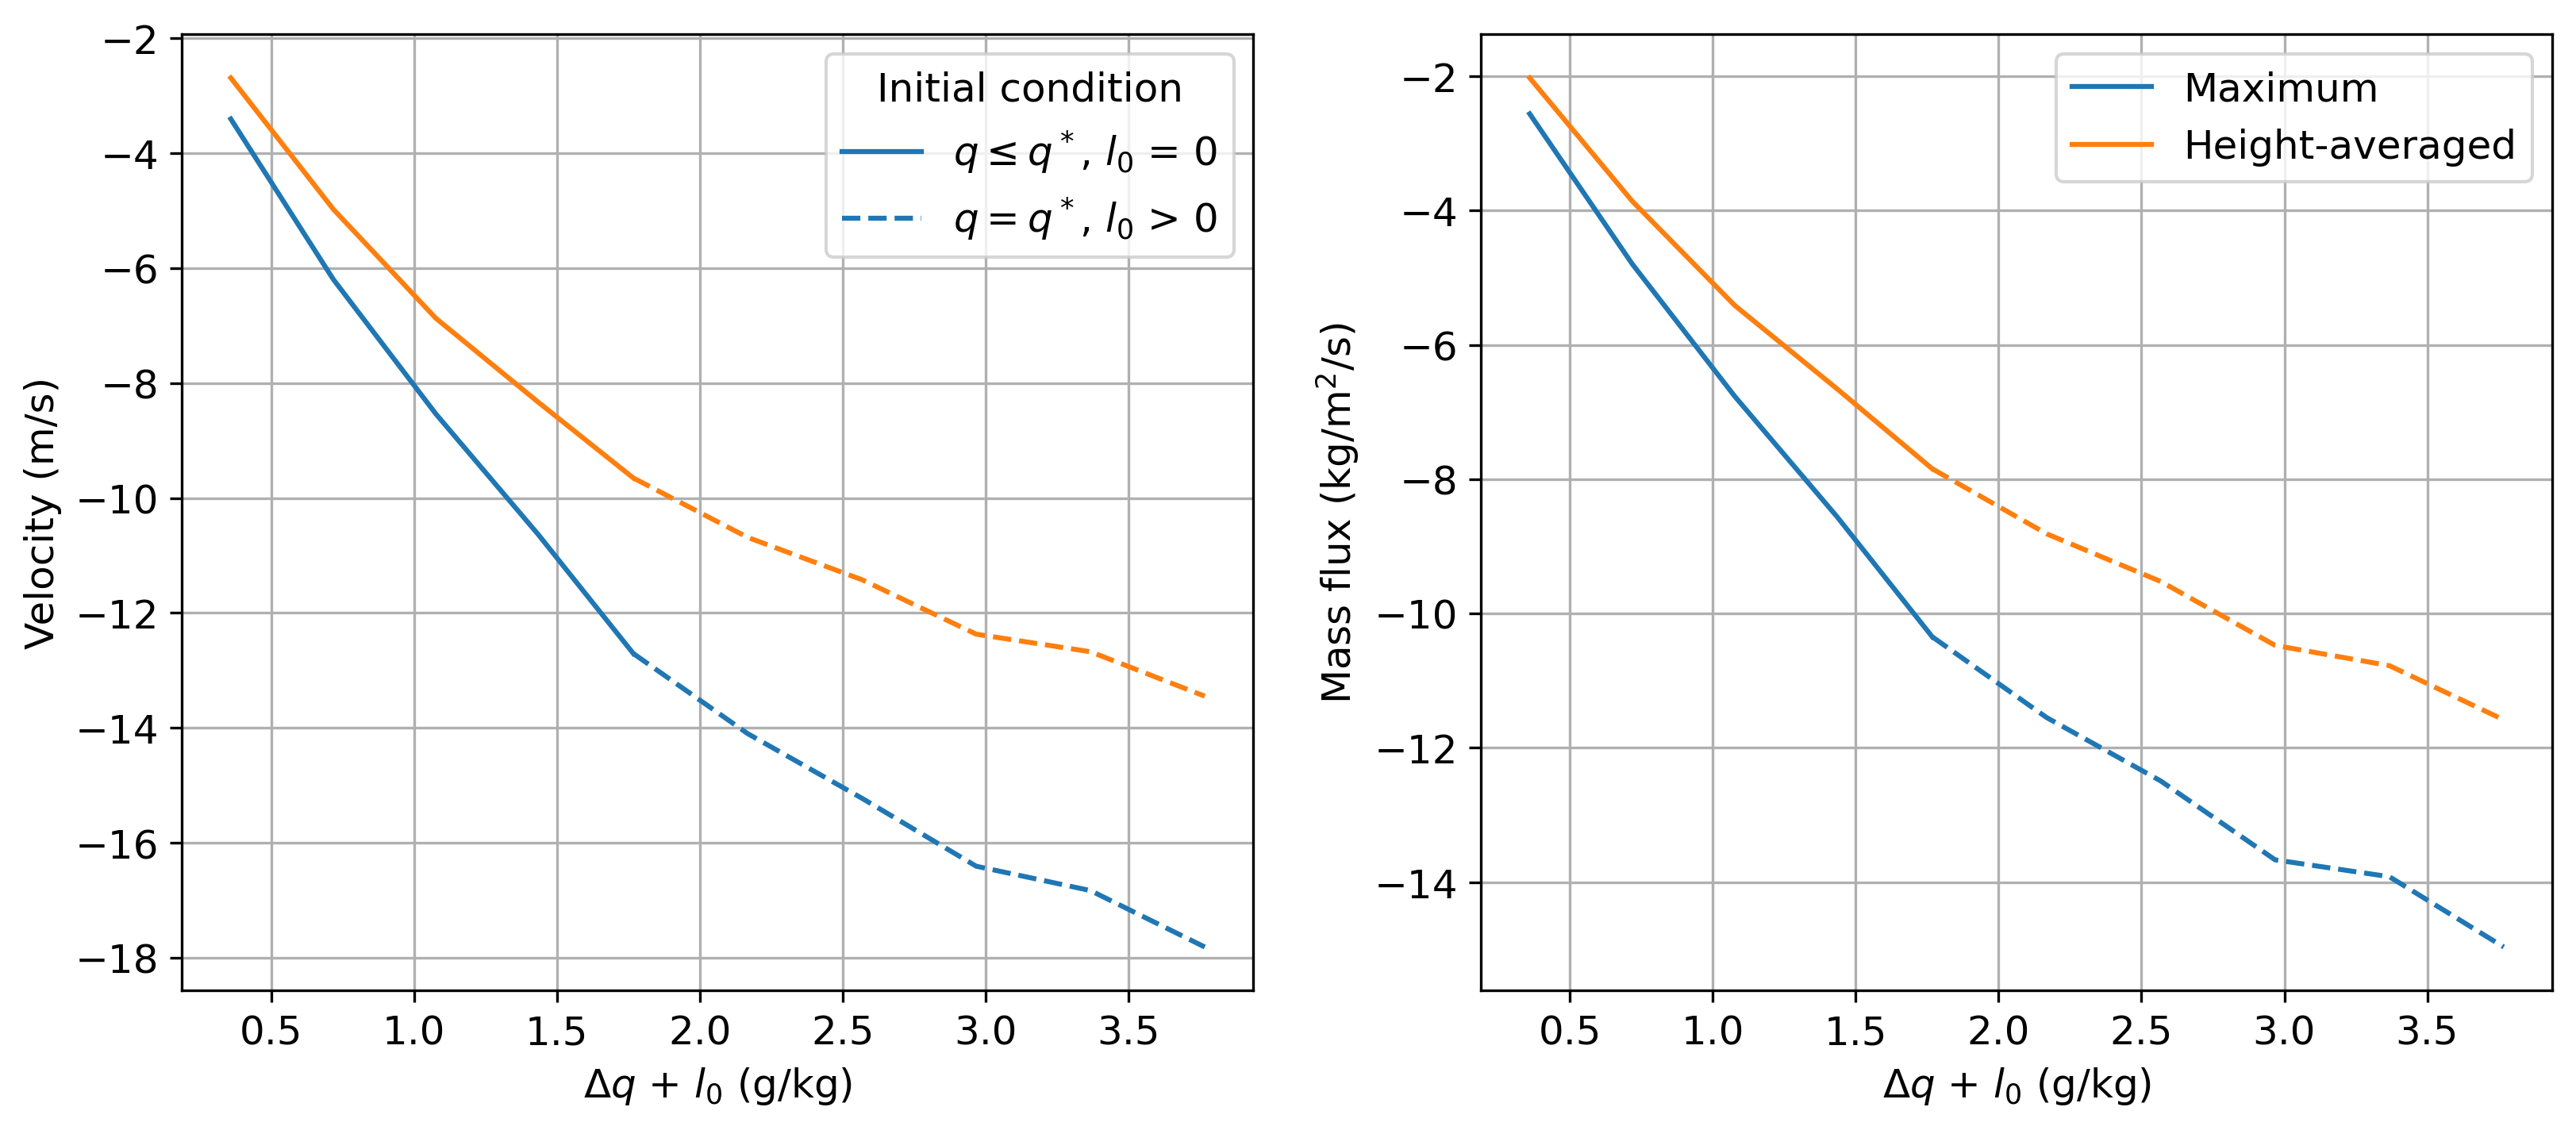
\includegraphics[width=0.8\linewidth]
		{figures/20211026_experiments_sydney/initial_conditions_vs_velocity}
	\caption{
		Maximum and height-averaged downdraft velocities computed as
		functions of the amount of water initially added. Dashed lines
		indicate that enough water is initially evaporated to saturate
		the parcel; the rest remains in the parcel as liquid and can
		evaporate during descent. The entrainment rate is fixed at
		$\SI{1}{\per\kilo\meter}$ and we use the Sydney sounding data.}
	\label{sydney_initial_conditions_vs_velocity}
\end{figure}

\begin{figure}[ht]
	\centering
	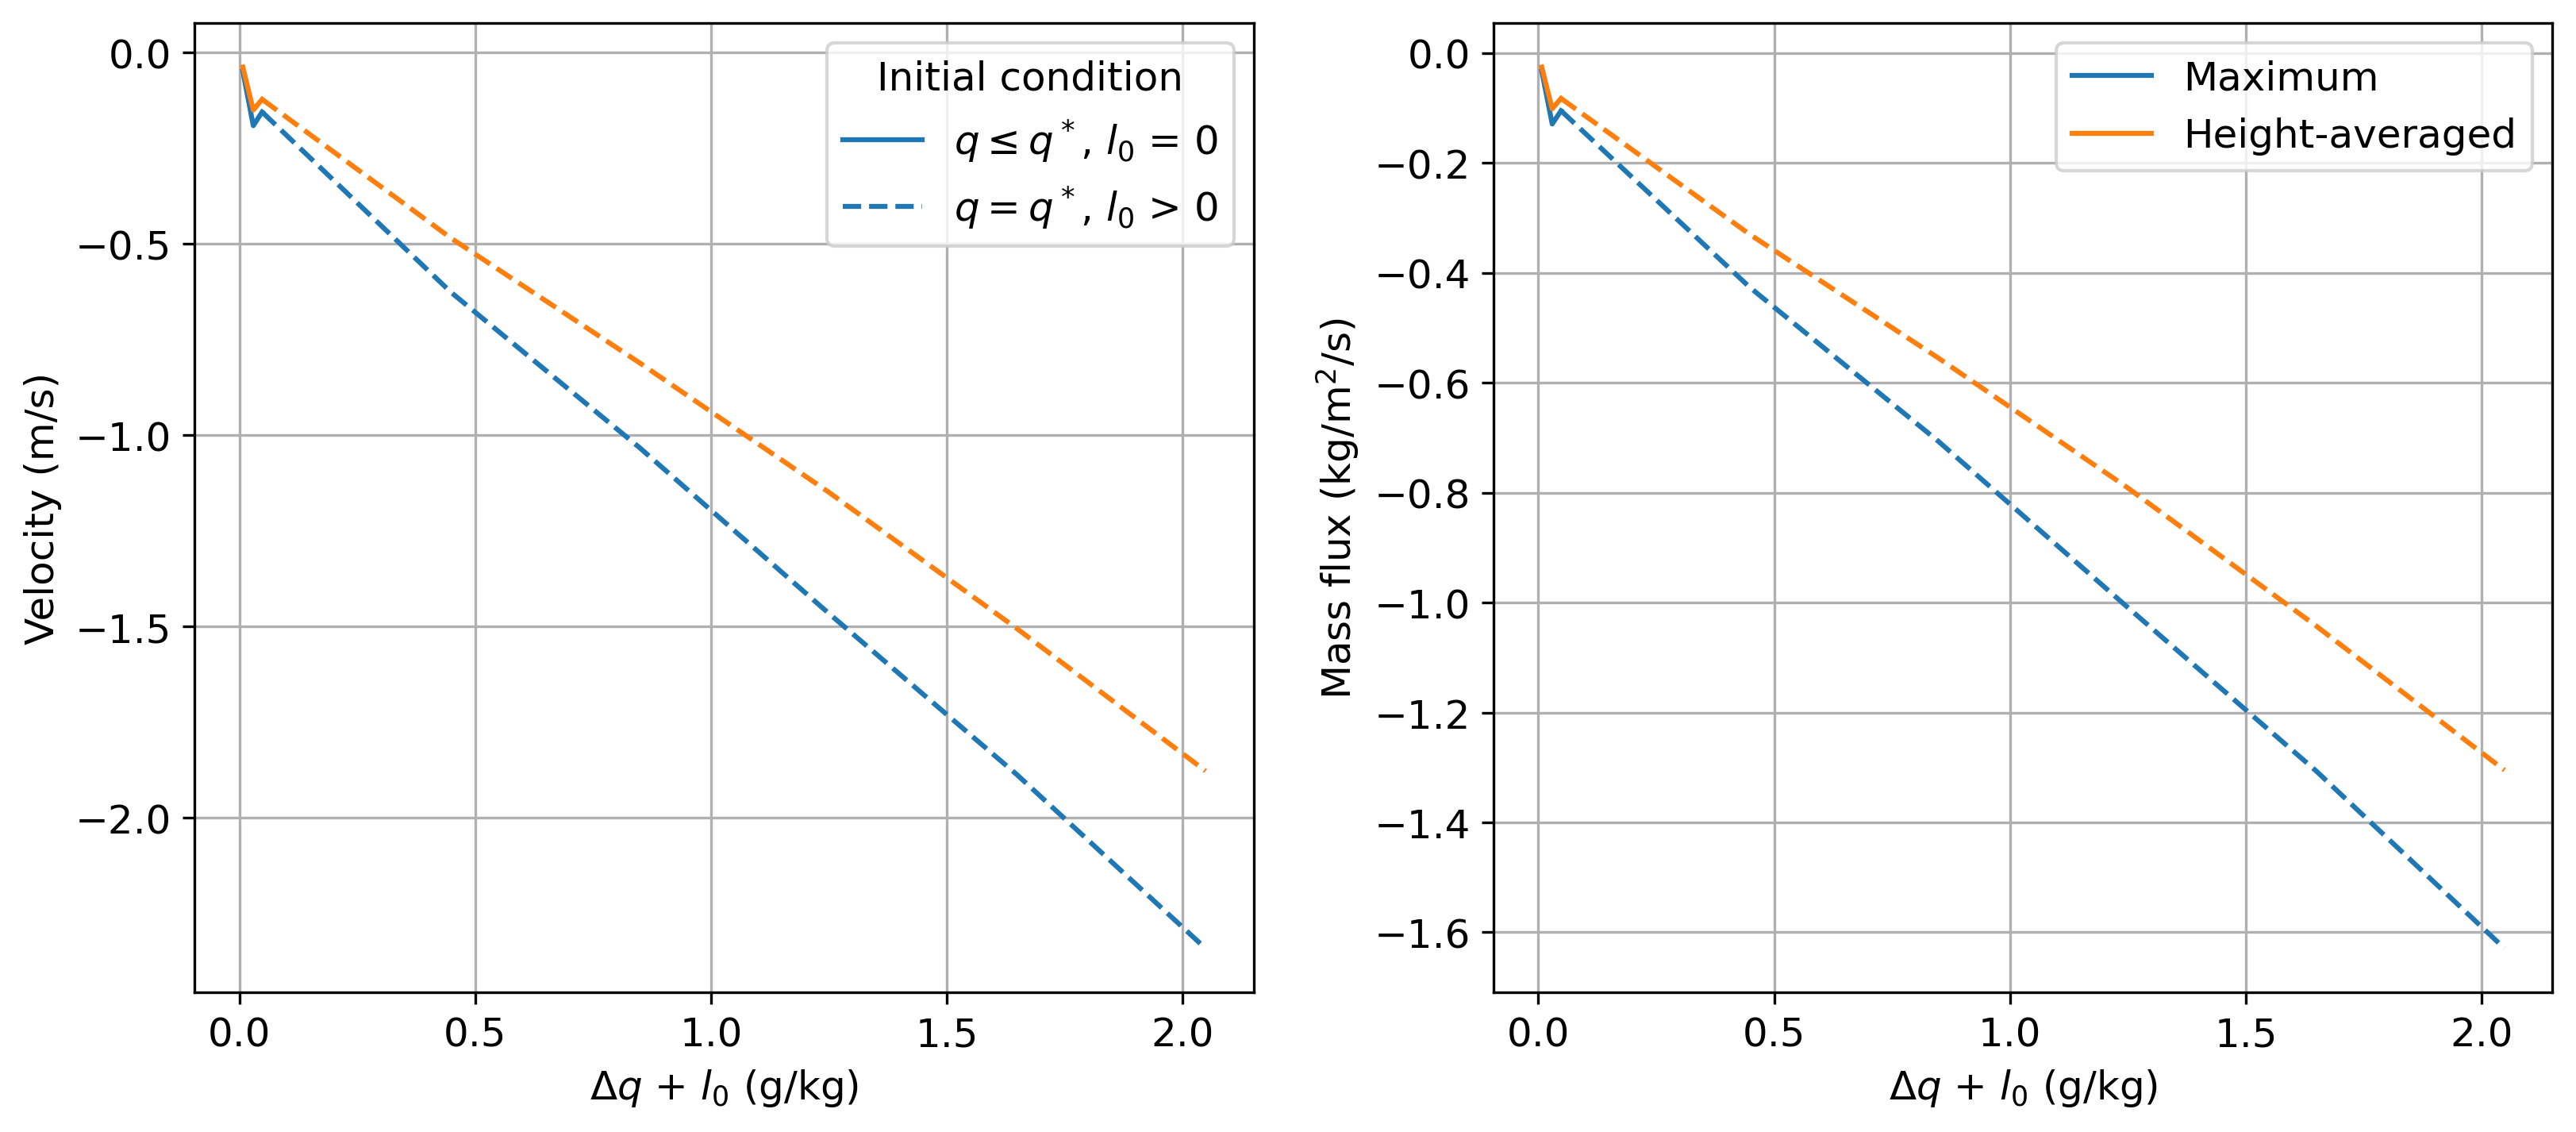
\includegraphics[width=0.8\linewidth]
		{figures/20211027_experiments_singapore/initial_conditions_vs_velocity}
	\caption{
		The result shown in Figure \ref{sydney_initial_conditions_vs_velocity},
		now using the Singapore sounding data.}
	\label{singapore_initial_conditions_vs_velocity}
\end{figure}

% \clearpage
% \printbibliography

\end{document}